\documentclass[pdflatex, ngerman]{beamer}

\usepackage[T1]{fontenc}
\usepackage[utf8]{inputenc}
%~ \usepackage{ngerman}
%~ \usepackage[babel]{csquotes}
%~ \usepackage{cite}
\usepackage{hyperref}
%~ \usepackage{color}
%~ \usepackage{listings}
%~ \usepackage{amsmath,amsfonts,amssymb}
\usepackage{graphicx}

%~ because tikz rocks
%~ \usepackage{tikz}
%~ \usetikzlibrary{calc,decorations.pathmorphing,patterns}

\usepackage{MyriadPro}
\usepackage{MinionPro}

%~ \usetheme{Amsterdam}
\DeclareOptionBeamer{compress}{\beamer@compresstrue}
\ProcessOptionsBeamer

\mode<presentation>

\useoutertheme{infolines}
\useinnertheme{rectangles}
\usecolortheme{whale}
\usecolortheme{orchid}

\definecolor{beamer@blendedblue}{rgb}{0.137,0.466,0.741}

\setbeamercolor{structure}{fg=beamer@blendedblue}
\setbeamercolor{titlelike}{parent=structure}
\setbeamercolor{frametitle}{fg=black}
\setbeamercolor{title}{fg=black}
\setbeamercolor{item}{fg=black}

\beamertemplatenavigationsymbolsempty

\title[Server NAS]{Server -- NAS}
\subtitle[Kurzform]{Private Sicherheitskopien vor Hardwarefehlern, \\Softwarefehlern und dem BKA schützen}
\author[Moritz Schlarb]{Moritz Schlarb}
\institute[JGU Mainz]{Institut für Informatik\\ Johannes Gutenberg-Universität Mainz}
\date[08.01.2013]{08. Januar 2013}
\subject{Learn Linux the Hard Way}
\keywords{RAID, LVM, LUKS, CIFS, Samba, NFS, rsync, }

\titlegraphic{
\includegraphics[scale=0.1]{logo}}

\setcounter{tocdepth}{2}
\begin{document}

\frame{
	\titlepage
}

\frame{
	\frametitle{Inhaltsverzeichnis}
	\tableofcontents
}

\begin{frame}{Easy vs. Awesome}
\begin{columns}
\column{.45\textwidth}
\begin{block}{\textbf{Easy:} \\ D-Link DNS-320}<1->
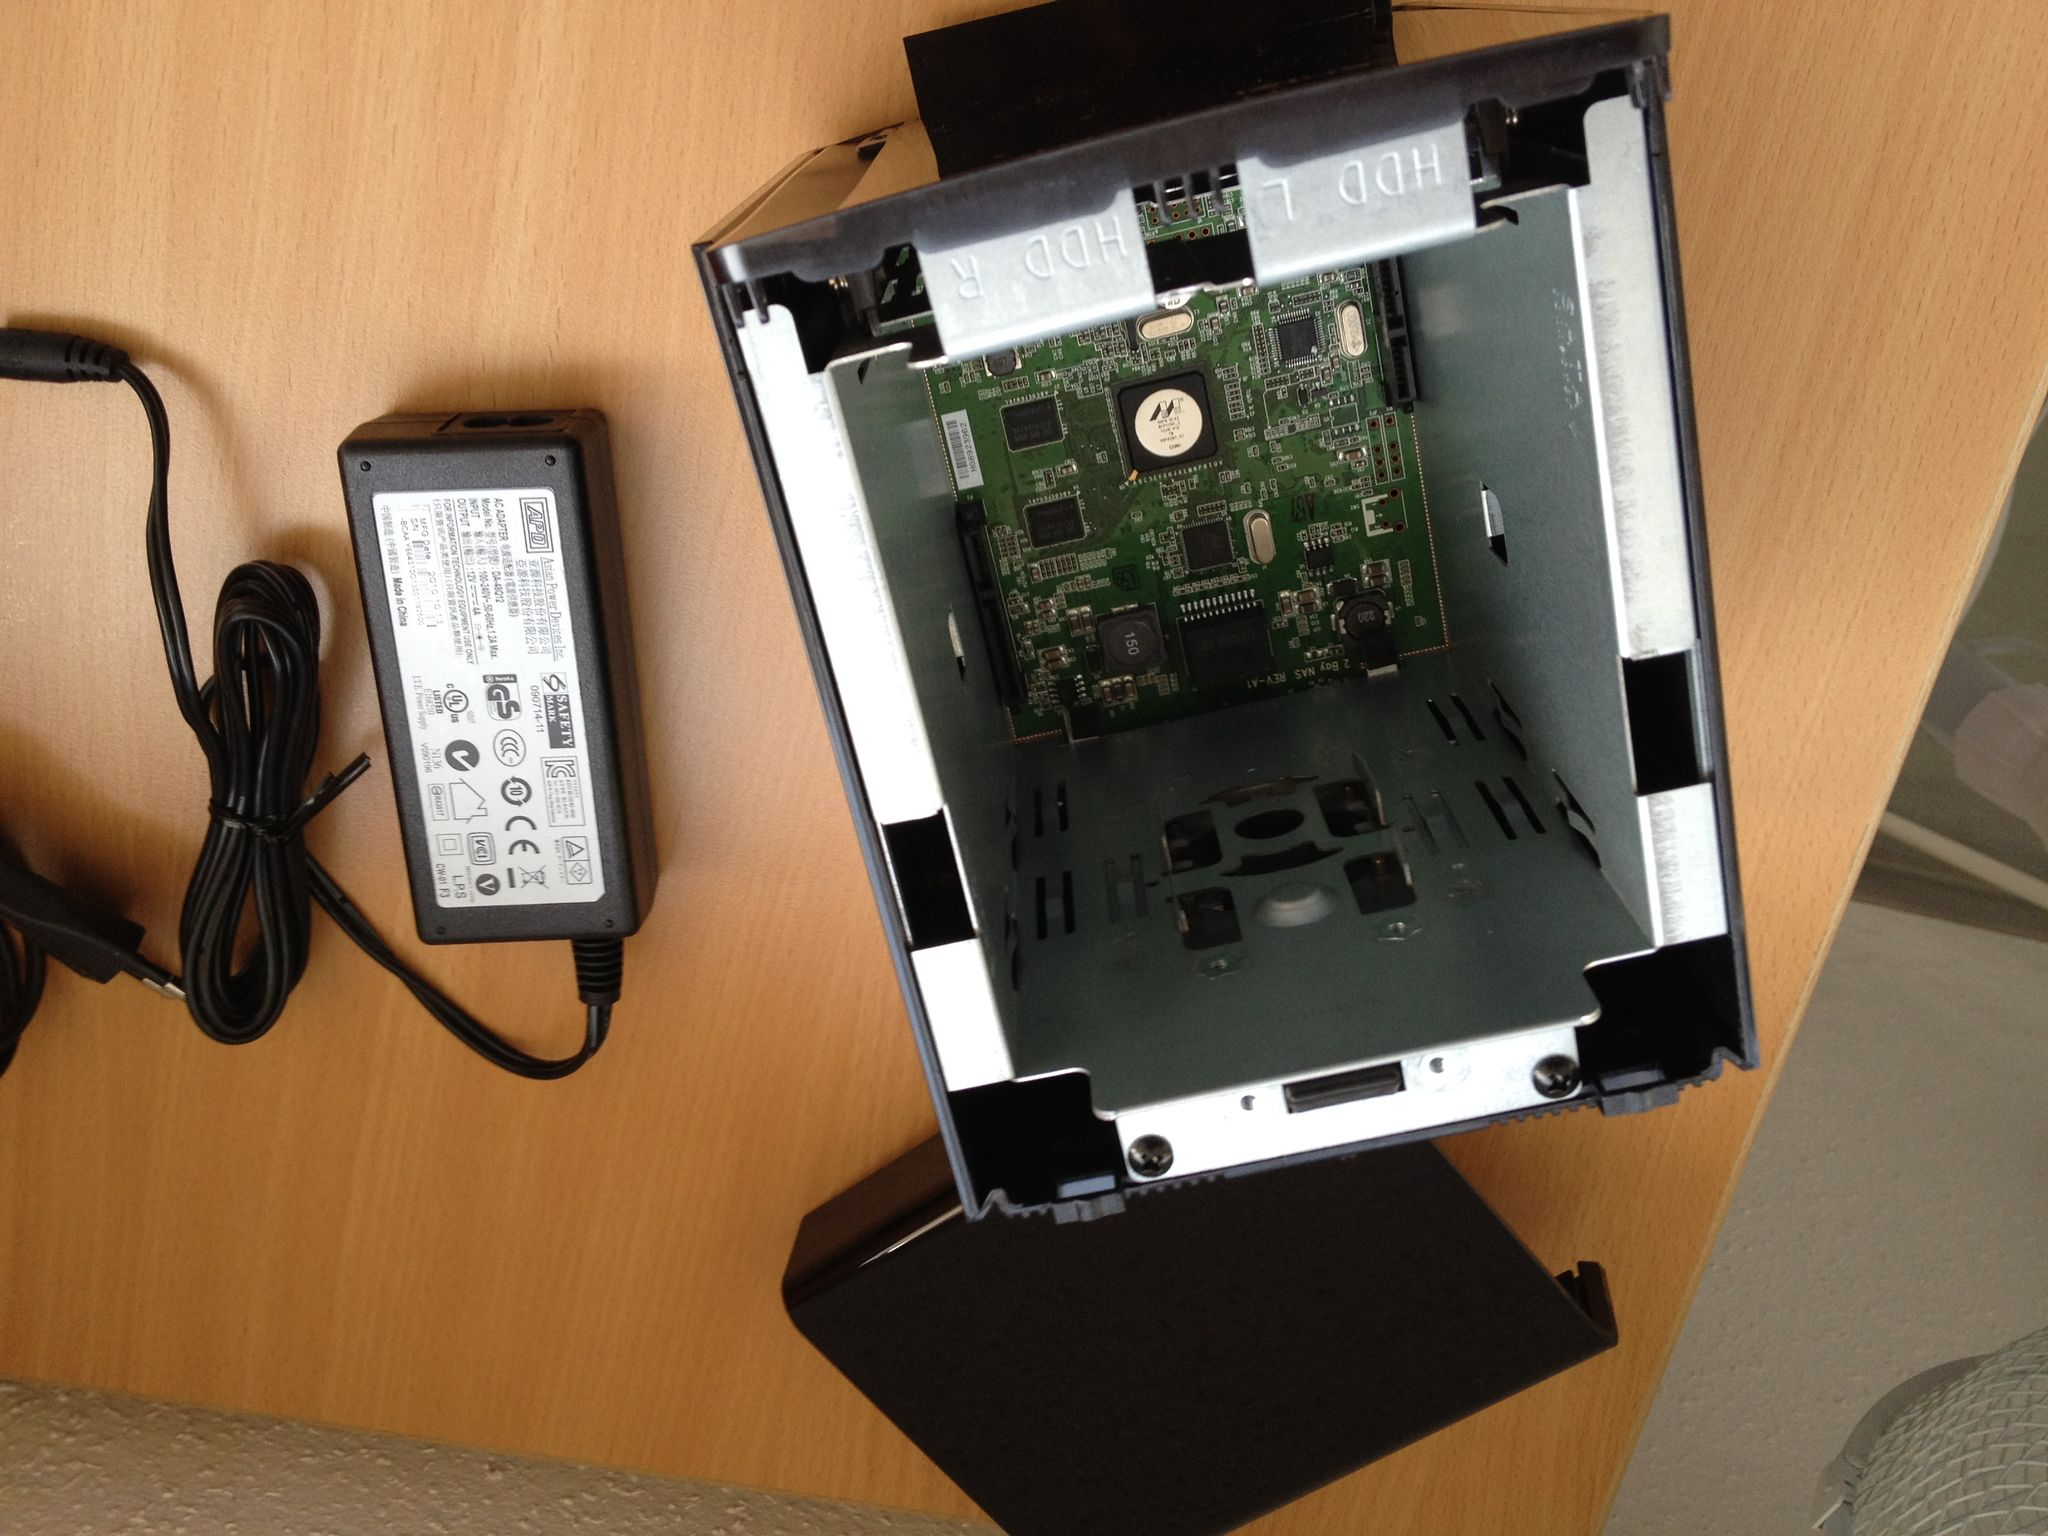
\includegraphics[width=\columnwidth,angle=180]{dns320_.jpg}
\begin{footnotesize}
  \begin{itemize}
    \item \textbf{CPU:} Marvell 88F6281, \\ 800MHz, ARMv5
    \item \textbf{RAM:} 128 MB
    \item \textbf{SATA:} 2x SATA II
  \end{itemize}
\end{footnotesize}
\end{block}
\column{.45\textwidth}
\begin{block}{\textbf{Awesome:} \\ HP Proliant Microserver N40L}<2->
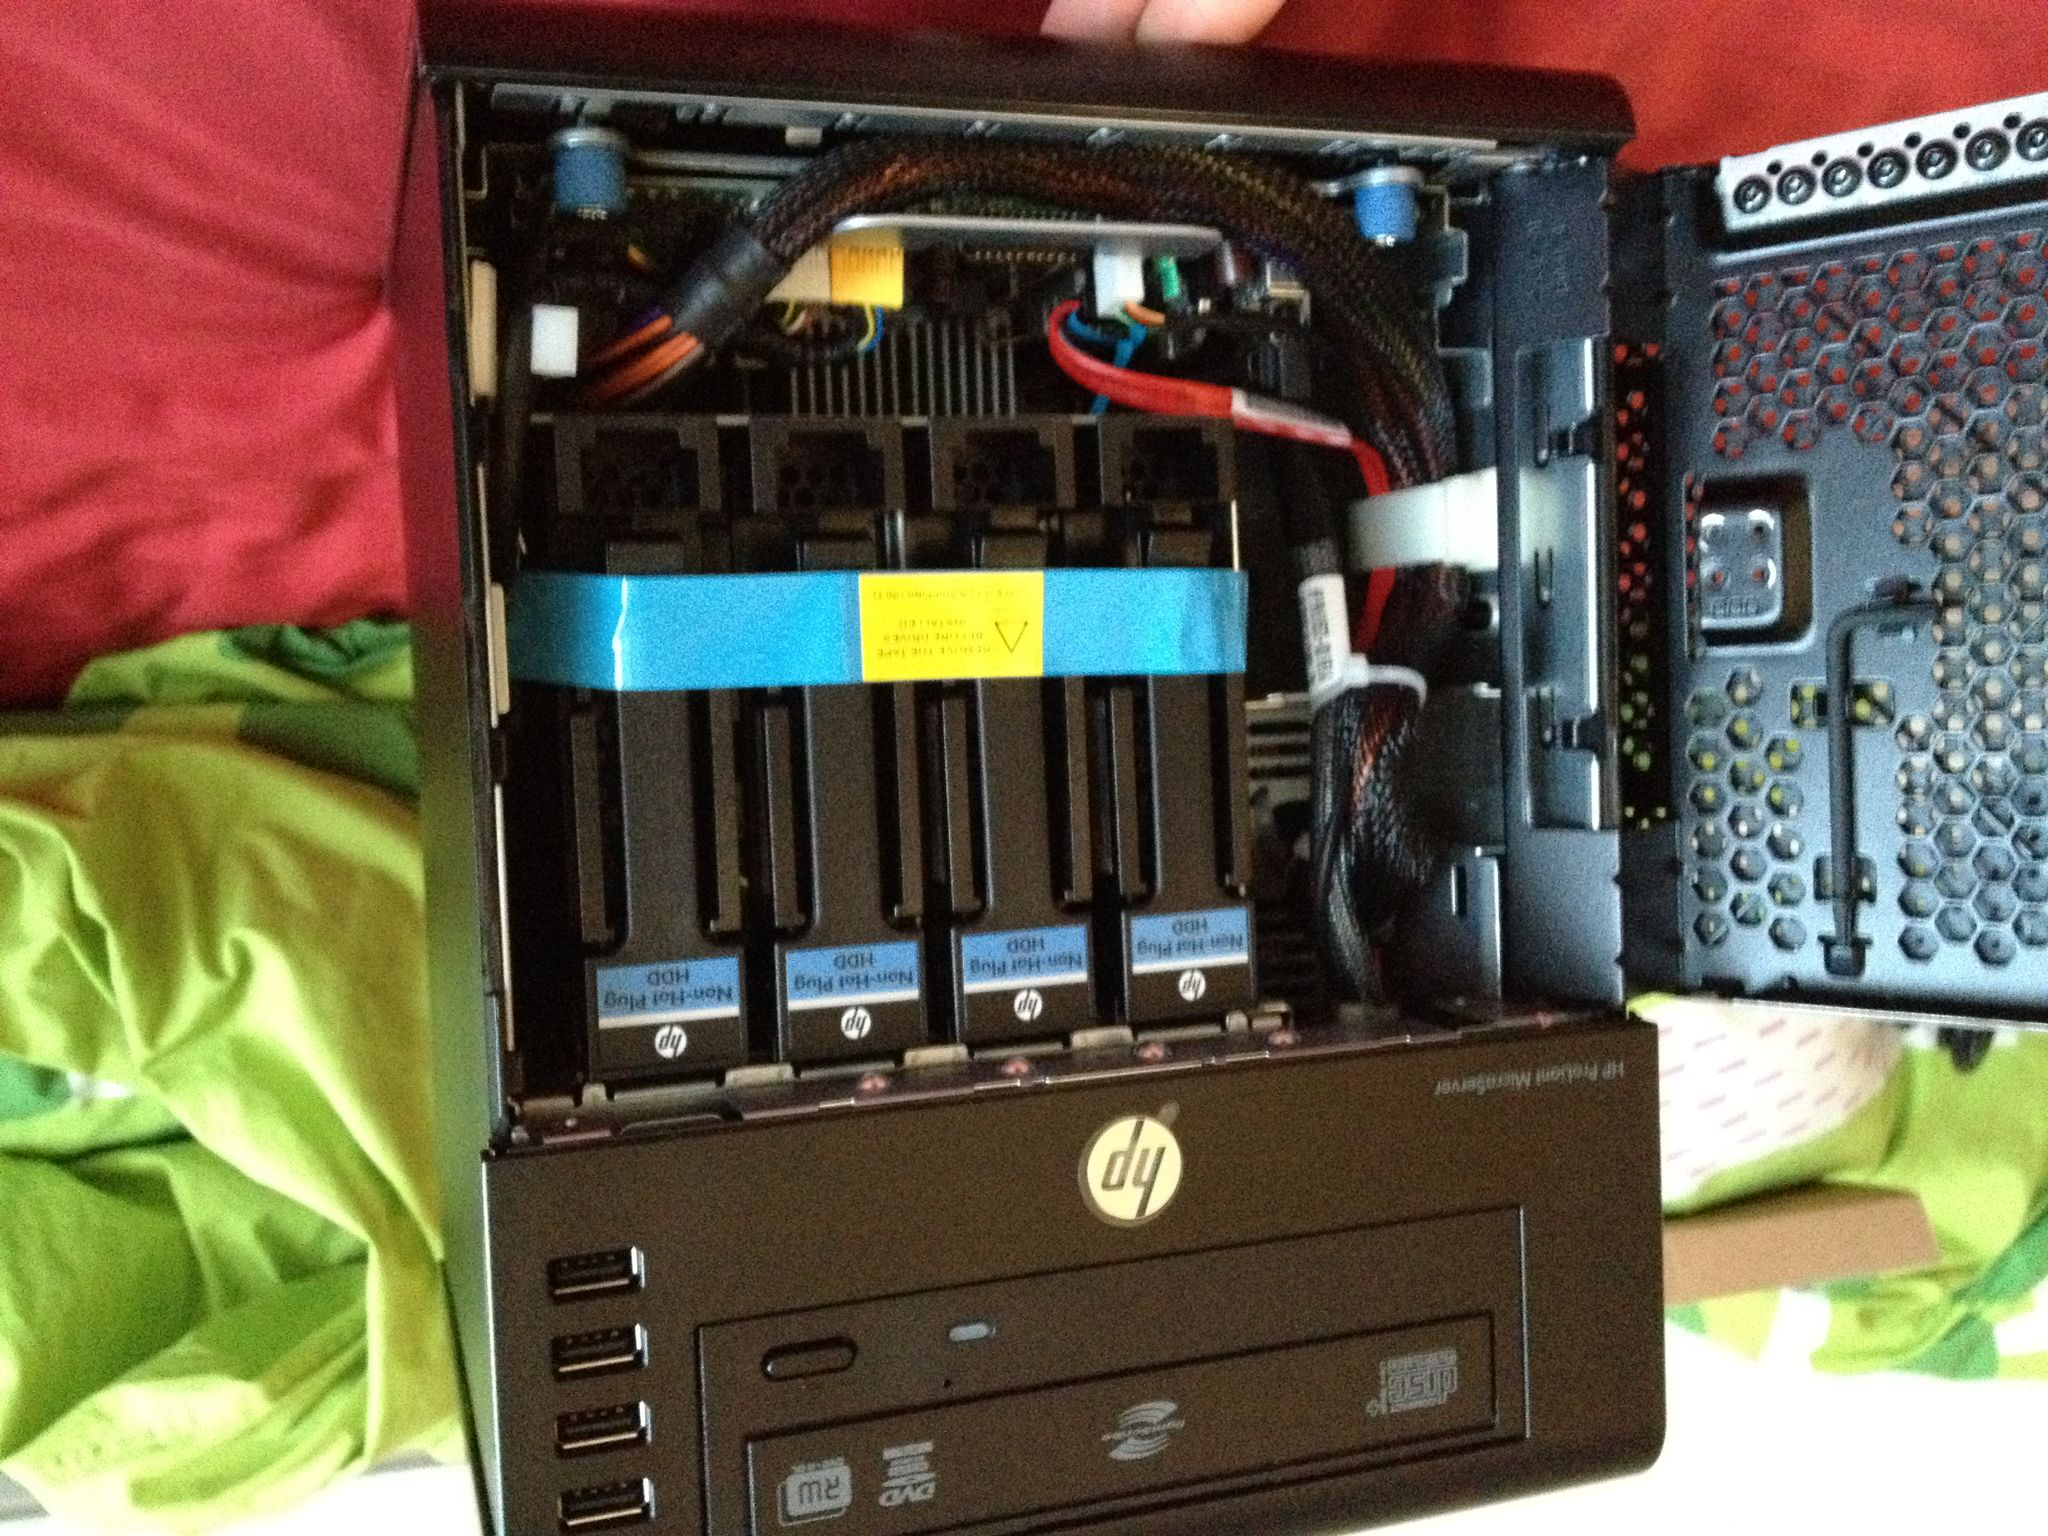
\includegraphics[width=\columnwidth,angle=180]{n40l_.jpg}
\begin{footnotesize}
  \begin{itemize}
    \item \textbf{CPU:} {AMD Turion II Neo N40L}, \\ 2x 1,5 GHz, AMD64
    \item \textbf{RAM:} 4 GB
    \item \textbf{SATA:} 5x SATA II
  \end{itemize}
\end{footnotesize}
\end{block}
\end{columns}
\end{frame}

\section{Blick über den Tellerrand}

\subsection{UNIX}

\begin{frame}{UNIX}
\begin{block}{UNIX Family Tree}
	\centering\colorbox{white}{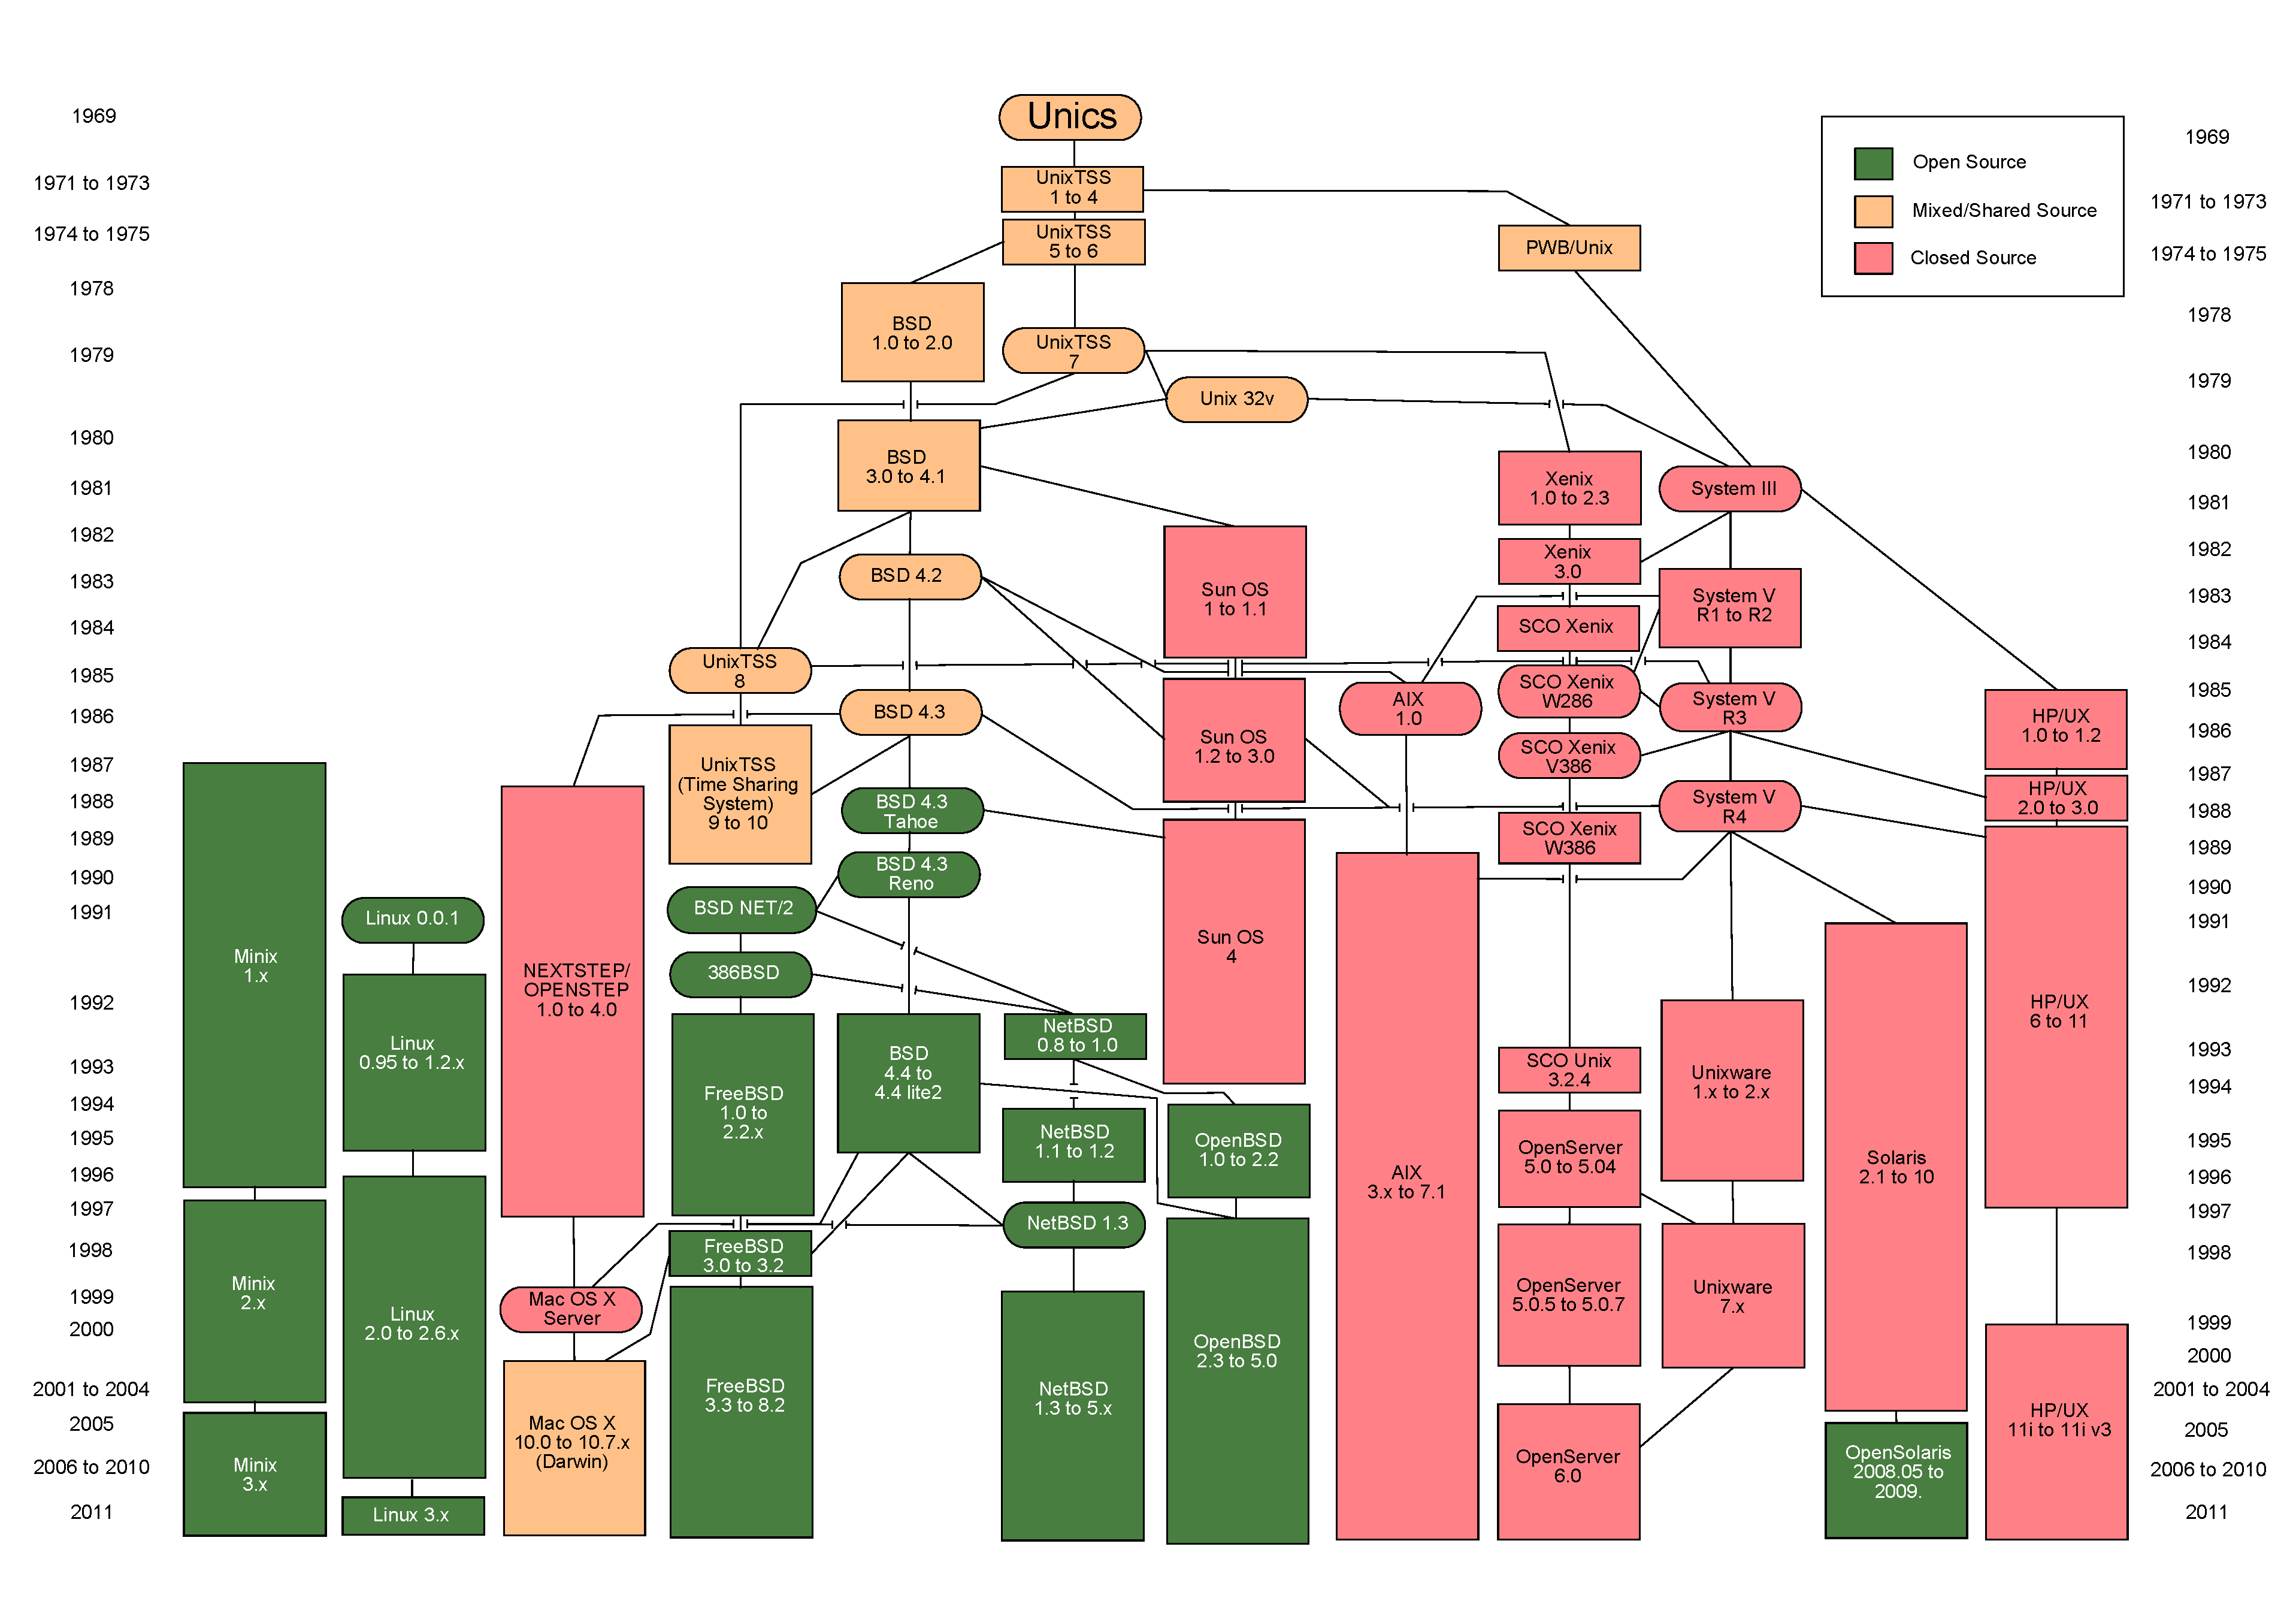
\includegraphics[width=0.8\columnwidth]{Unix_history-simple}}

   	{\tiny File:Unix history-simple.svg, Revision as of 17:10, 23 June 2012 --
   	Source: Wikimedia Commons, License: CC-BY-SA-3.0
   	%~ \\ URL: \url{http://commons.wikimedia.org/w/index.php?title=File:Unix_history-simple.svg&oldid=73135501}
   	}
\end{block}
\end{frame}

\subsection{Lizenzen}

\begin{frame}{GPL vs. the Rest}
\begin{columns}
\column{.45\textwidth}
\centering
\includegraphics[width=0.5\columnwidth]{Official_gnu}
\column{.45\textwidth}
\centering
\includegraphics[width=0.5\columnwidth]{GPLv3_Logo}
\end{columns}
\begin{columns}
\column{.45\textwidth}
\begin{block}{GPL-kompatibel}
  \begin{itemize}
    \item LGPL
    \item BSD-2, BSD-3
    \item MIT
  \end{itemize}
\end{block}
\column{.45\textwidth}
\begin{block}{Nicht GPL-kompatibel}
  \begin{itemize}
    \item BSD-4
    \item CDDL-1.0
    \item Apache-2.0
    \item MPL-2.0
    \item EPL-1.0
  \end{itemize}
\end{block}
\end{columns}
\end{frame}

\section{Virtualisierung mit Bordmitteln}

\subsection{KVM}

\begin{frame}{KVM}{Kernel-based Virtual Machine}
\centering
\includegraphics[width=0.5\columnwidth]{kvmbanner-logo2}
\begin{block}{}
  \begin{itemize}
    \item Benötigt Prozessor-Unterstützung für Hardware-Virtualisierung: \\
    	Intel (Intel VT) oder AMD (AMD-V) \\
        \texttt{\$ egrep 'vmx|svm' /proc/cpuinfo}
    \item Hypervisor
    \item Paravirtualisierung durch Virtio
  \end{itemize}
\end{block}
\end{frame}

\begin{frame}{QEMU}
\begin{block}{}
  \begin{itemize}
    \item ``Quick Emulator''
    \item Kann verschiedene Prozessorarchitekturen emulieren: \\
		i386, x86\_64, arm, mips, ppc
    \item Emulator für Geräte (Festplatten, Netzwerk-, Sound- und Grafikkarten)
  \end{itemize}
\end{block}
\end{frame}

\subsection{libvirt}

\begin{frame}{libvirt}
\centering
\includegraphics[width=0.5\columnwidth]{Libvirt_logo}
\begin{columns}
\column{\textwidth}
\begin{block}{}
  \begin{itemize}
    \item Bibliothek/API/Daemon zur Konfiguration/Steuerung von verschiedenen Virtualisierungsumgebungen
  \end{itemize}
\end{block}
\end{columns}
\end{frame}

\subsection{virt-manager}

\begin{frame}{virt-manager}
\centering
\includegraphics[width=0.5\columnwidth]{virt-manager_logo}
\begin{block}{}
  \begin{itemize}
    \item Grafisches Frontend für libvirt
  \end{itemize}
\end{block}
\end{frame}

\section{Partitionierung like a Boss}

\subsection{RAID}

\begin{frame}{RAID}{Redundant Array of Inexpensive Disks}

\end{frame}

\subsection{LVM}

\begin{frame}{LVM}{Logical Volume Manager}

\end{frame}

\subsection{LUKS}

\begin{frame}{LUKS}{Linux Unified Key Setup}

\end{frame}

\subsection{ZFS}

\begin{frame}{ZFS}{ZFS on Linux}

%~ https://mthode.org/gentoo-hardened-zfs-rootfs-with-dm-cryptluks/

\begin{alertblock}{Warnung}
	Don't try this at home!
\end{alertblock}

\begin{block}{}
	\url{http://zfsonlinux.org/}
\end{block}

\end{frame}

\section{Verteilte Dateisysteme}

\subsection{CIFS (Samba)}

\begin{frame}{CIFS}{Common Internet File System}

%~ \begin{columns}
%~ \column{.45\textwidth}
\begin{block}{}
  \begin{itemize}
    \item Nachfolger von SMB (Server Message Block) -- Namensgeber für Samba
  \end{itemize}
\end{block}
%~ \end{columns}

\end{frame}

\subsection{NFS}

\begin{frame}{NFS}{Network File System}

\end{frame}

%~ \section{Tools}

% ~\subsection{rsync}

%~ \begin{frame}
%~ \frametitle{Tikz Awesomeness!!!!!111einself}
%~
%~ \pgfdeclaredecoration{penciline}{initial}{
    %~ \state{initial}[width=+\pgfdecoratedinputsegmentremainingdistance,
    %~ auto corner on length=1mm,]{
        %~ \pgfpathcurveto%
        %~ {% From
            %~ \pgfqpoint{\pgfdecoratedinputsegmentremainingdistance}
                      %~ {\pgfdecorationsegmentamplitude}
        %~ }
        %~ {%  Control 1
        %~ \pgfmathrand
        %~ \pgfpointadd{\pgfqpoint{\pgfdecoratedinputsegmentremainingdistance}{0pt}}
                    %~ {\pgfqpoint{-\pgfdecorationsegmentaspect
                     %~ \pgfdecoratedinputsegmentremainingdistance}%
                               %~ {\pgfmathresult\pgfdecorationsegmentamplitude}
                    %~ }
        %~ }
        %~ {%TO
        %~ \pgfpointadd{\pgfpointdecoratedinputsegmentlast}{\pgfpoint{1pt}{1pt}}
        %~ }
    %~ }
    %~ \state{final}{}
%~ }
%~
%~ \begin{center}
%~ \begin{tikzpicture}[decoration=penciline, decorate]
%~ \draw[decorate] (-2,-2) grid[step=1cm] (4,4);
%~ \draw[decorate] (0 , 0) node[auto] {Poodle};
%~ \end{tikzpicture}
%~ \end{center}
%~ \end{frame}

\end{document}
